\documentclass[a4paper,oneside,12pt]{report}
\usepackage{fontspec}
\usepackage{setspace}
\usepackage{amsmath}
\usepackage{titling}
\usepackage{geometry}
\usepackage{listings}
\usepackage{xcolor}
\usepackage{float}
\usepackage{graphicx}
\usepackage{xurl}
\usepackage{hyperref}
\usepackage{indentfirst}
\usepackage{fancyhdr}
\usepackage{tocloft}
\usepackage{bookmark}
\usepackage{booktabs}
\usepackage{array}
\usepackage{caption}
\usepackage{microtype}
\usepackage{titlesec}
\titleformat{\chapter}[block]{\LARGE\bfseries}{}{0pt}{}
\titlespacing*{\chapter}{0pt}{0pt}{18pt}

\emergencystretch=3em
\hfuzz=1.5pt

\setmainfont{texgyretermes-regular.otf}[
    BoldFont=texgyretermes-bold.otf,
    ItalicFont=texgyretermes-italic.otf,
    BoldItalicFont=texgyretermes-bolditalic.otf
]
\onehalfspacing
\geometry{left=3cm, right=2.5cm, top=2cm, bottom=2.5cm}
\sloppy

\definecolor{codegreen}{rgb}{0,0.6,0}
\definecolor{codegray}{rgb}{0.5,0.5,0.5}
\definecolor{codepurple}{rgb}{0.58,0,0.82}
\definecolor{backcolour}{rgb}{0.96,0.96,0.94}
\definecolor{darkblue}{rgb}{0,0,0.6}

\lstdefinestyle{commonstyle}{
    backgroundcolor=\color{backcolour},
    breakatwhitespace=false,
    breaklines=true,
    captionpos=b,
    keepspaces=true,
    numbers=left,
    numbersep=5pt,
    showspaces=false,
    showstringspaces=false,
    showtabs=false,
    tabsize=2,
    frame=single,
    basicstyle=\ttfamily\footnotesize,
    numberstyle=\tiny\color{codegray},
    columns=flexible,
    postbreak=\mbox{\textcolor{red}{$\hookrightarrow$}\space},
    breakindent=0pt,
    breakautoindent=false
}
\lstdefinestyle{bashstyle}{
    style=commonstyle,
    language=bash,
    commentstyle=\color{codegreen},
    keywordstyle=\color{darkblue},
    stringstyle=\color{codepurple}
}
\lstdefinestyle{yamlstyle}{
    style=commonstyle,
    commentstyle=\color{codegreen},
    keywordstyle=\color{darkblue},
    stringstyle=\color{codepurple}
}
\lstdefinestyle{dockerstyle}{
    style=commonstyle,
    commentstyle=\color{codegreen},
    keywordstyle=\color{darkblue},
    stringstyle=\color{codepurple}
}
\lstdefinestyle{phpstyle}{
    style=commonstyle,
    language=PHP,
    commentstyle=\color{codegreen},
    keywordstyle=\color{darkblue},
    stringstyle=\color{codepurple}
}
\lstdefinestyle{jsonstyle}{
    style=commonstyle,
    commentstyle=\color{codegreen},
    keywordstyle=\color{darkblue},
    stringstyle=\color{codepurple}
}

\newcommand{\customfbox}[1]{%
  \setlength{\fboxsep}{0pt}%
  \setlength{\fboxrule}{0.5pt}%
  \fbox{#1}%
}

\renewcommand{\figurename}{Gambar}
\renewcommand{\contentsname}{Daftar Isi}
\renewcommand{\bibname}{Daftar Pustaka}
\renewcommand{\thefigure}{\arabic{figure}}
\renewcommand{\thetable}{\arabic{table}}
\renewcommand{\tablename}{Tabel}
\renewcommand{\lstlistingname}{Listing}
\AtBeginDocument{\renewcommand{\thelstlisting}{\arabic{lstlisting}}}
\hypersetup{
    colorlinks=true,
    linkcolor=black,
    citecolor=black,
    filecolor=black,
    urlcolor=blue
}

\pagestyle{fancy}
\fancyhf{}
\fancyfoot[C]{\thepage}
\renewcommand{\headrulewidth}{0pt}
\fancypagestyle{plain}{
    \fancyhf{}
    \fancyfoot[C]{\thepage}
    \renewcommand{\headrulewidth}{0pt}
}

\setlength{\cftbeforetoctitleskip}{0pt}
\setlength{\cftaftertoctitleskip}{20pt}
\renewcommand{\cfttoctitlefont}{\hfill\Large\bfseries}
\renewcommand{\cftaftertoctitle}{\hfill}

\renewcommand{\cftchapleader}{\cftdotfill{\cftdotsep}}
\renewcommand{\cftsecleader}{\cftdotfill{\cftdotsep}}
\renewcommand{\cftsubsecleader}{\cftdotfill{\cftdotsep}}

\renewcommand{\thechapter}{}
\renewcommand{\chaptername}{}
\renewcommand{\thesection}{\arabic{chapter}.\arabic{section}}
\renewcommand{\thesubsection}{\thesection.\arabic{subsection}}
\setlength{\cftchapindent}{0em}
\setlength{\cftsecindent}{2em}
\setlength{\cftsubsecindent}{4em}
\setlength{\cftchapnumwidth}{0em}
\setlength{\cftsecnumwidth}{2.8em}
\setlength{\cftsubsecnumwidth}{3.2em}
\renewcommand{\cftchappresnum}{}
\renewcommand{\cftchapaftersnum}{}
\newcommand{\tocboldsection}[1]{%
  \protect\renewcommand{\protect\cftchapfont}{\protect\bfseries}%
  #1%
  \protect\renewcommand{\protect\cftchapfont}{}%
}



\begin{document}

\newgeometry{left=2.5cm, right=2.5cm, top=2.5cm, bottom=2.5cm}
\begin{titlepage}
    \centering
    \vspace*{0.2cm}
    {\Large\bfseries LAPORAN PRAKTIKUM KEPL}\\[0.3cm]
    {\large\bfseries TUGAS 4: DOCKERFILE, .DOCKERIGNORE, DAN BUKTI CACHE BUILD APLIKASI LARAVEL}\\[1.2cm]

    
\includegraphics[width=0.38\textwidth]{images/UGM.png}\\[1cm]

    {\large\bfseries Disusun oleh:}\\[0.2cm]
    {\bfseries Hafidz Rizqullah Prasetya}\\[0.1cm]
    {\bfseries NIM: 24/535493/SV/24243}\\[0.1cm]
    {\bfseries Kelas: PL5A1}\\[1cm]

    {\large Dosen Pengampu:\\[0.2cm]
    \bfseries Galih Damaraji, S.Kom., M.Cs.}\\[0.8cm]

    \vfill
    {\bfseries PROGRAM STUDI SARJANA TERAPAN\\PENGEMBANGAN PERANGKAT LUNAK TERDISTRIBUSI\\DEPARTEMEN TEKNIK ELEKTRO DAN INFORMATIKA\\SEKOLAH VOKASI\\UNIVERSITAS GADJAH MADA\\YOGYAKARTA\\2026}
\end{titlepage}
\restoregeometry

\thispagestyle{empty}
\clearpage
\stepcounter{page}
\thispagestyle{empty}

\addcontentsline{toc}{chapter}{Daftar Isi}
\tableofcontents
\clearpage

\pagenumbering{arabic}
\setcounter{page}{3}

\chapter{Tujuan dan Lingkup Praktikum}

\section{Tujuan Praktikum}
Setelah mengerjakan Tugas 4, mahasiswa diharapkan dapat:
\begin{enumerate}
    \item menulis Dockerfile untuk aplikasi Laravel di repositori \texttt{evolusi-pl-NIM};
    \item membuat \texttt{.dockerignore} yang minimal mengecualikan \texttt{node\_modules}, \texttt{vendor}, \texttt{.git}, dan \texttt{.env};
    \item mengurutkan instruksi Dockerfile supaya \texttt{composer.json} dan \texttt{composer.lock} disalin dan dipasang sebelum kode aplikasi;
    \item membuktikan cache build bekerja lewat tiga kali build: build awal, build ulang tanpa perubahan, dan build setelah satu huruf kode diubah;
    \item menjalankan container, membukanya dari browser, dan menunjukkan output \texttt{docker ps};
    \item memanggil API dari luar container dengan Postman sampai mendapat status 200 dan isi JSON.
\end{enumerate}

\section{Batasan Masalah dan Repositori Kode}
Tugas ini memakai repositori yang sama dengan tugas-tugas sebelumnya, yaitu aplikasi daftar tugas kuliah berbasis Laravel:
\begin{center}
    \url{https://github.com/hafidzrizqullahprasetya/evolusi-pl-535493}
\end{center}
\texttt{Dockerfile} dan \texttt{.dockerignore} masuk ke branch \texttt{main} lewat Pull Request \#16 (commit \texttt{439da82}). Dockerfile yang sama juga dipakai pada Tugas 5 tentang multi-stage build. Seluruh build dan pengujian di laporan ini dijalankan ulang di laptop pengerjaan (Ubuntu, Docker Engine 29.9.2, Buildx v0.38.1) pada 18 November 2026, sehingga waktu build di screenshot adalah hasil hari itu.

\clearpage

\chapter{Dasar Teori}

\section{Dockerfile dan Layer Image}
Dockerfile adalah daftar instruksi untuk membangun image. Instruksi seperti \texttt{RUN}, \texttt{COPY}, dan \texttt{ADD} masing-masing menghasilkan satu layer, dan layer-layer itu ditumpuk sesuai urutan instruksi \cite{dockerfile-ref}. Dengan \textit{multi-stage build}, satu Dockerfile bisa memiliki beberapa \texttt{FROM}. Tahap pertama dipakai untuk menyiapkan dependensi, lalu tahap akhir hanya mengambil hasil yang dibutuhkan lewat \texttt{COPY --from}.

\section{Cara Kerja Cache Build}
Saat build, Docker memeriksa setiap instruksi secara berurutan. Jika instruksi dan masukannya sama dengan build sebelumnya, layer lama dipakai ulang dan output build menandainya \texttt{CACHED}. Untuk \texttt{COPY}, yang dibandingkan adalah isi berkas yang disalin. Begitu satu layer berubah, semua instruksi sesudahnya ikut dijalankan ulang \cite{docker-cache}. Karena itu, langkah yang mahal dan jarang berubah, seperti memasang dependensi, sebaiknya ditaruh sebelum langkah yang sering berubah, seperti menyalin kode aplikasi.

\section{Build Context dan .dockerignore}
Perintah \texttt{docker build .} mengirim isi folder saat ini ke builder sebagai \textit{build context}. Berkas \texttt{.dockerignore} menyaring isi context itu dengan pola yang mirip \texttt{.gitignore}. Berkas yang dikecualikan tidak terkirim ke builder dan tidak bisa ikut tersalin oleh \texttt{COPY . .} \cite{docker-context}. Folder besar seperti \texttt{vendor} dan \texttt{node\_modules}, riwayat \texttt{.git}, serta berkas rahasia seperti \texttt{.env} biasanya dimasukkan ke sini.

\section{Publish Port dan Pengujian API}
Container punya jaringan sendiri. Agar layanan di dalamnya bisa dibuka dari host, port container perlu dipetakan ke port host dengan opsi \texttt{-p host:container} \cite{docker-ports}. Setelah itu, API bisa diuji dari luar container dengan Postman, yang menampilkan URL permintaan, status HTTP, waktu respons, dan isi balasan \cite{postman-request}.

\clearpage

\chapter[\texorpdfstring{\tocboldsection{Hasil dan Pembahasan}}{Hasil dan Pembahasan}]{Hasil dan Pembahasan}

Semua perintah di bab ini dijalankan dari akar repositori \texttt{evolusi-pl-535493}.

\section{Dockerfile Aplikasi Laravel (Soal 1)}
Listing \ref{lst:dockerfile} adalah Dockerfile di akar repositori. Tahap \texttt{builder} memakai image \texttt{composer:2.8.5} untuk memasang dependensi produksi. Tahap akhir memakai \texttt{php:8.4.26-cli-alpine}, memasang ekstensi \texttt{bcmath}, lalu mengambil folder \texttt{/app} dari tahap \texttt{builder}. Di tahap akhir, berkas \texttt{.env} dibuat dari \texttt{.env.example}, kunci aplikasi dibuat, migrasi dijalankan ke SQLite, dan kepemilikan folder diserahkan ke \texttt{www-data}. Container berjalan sebagai \texttt{www-data}, membuka port 8000, dan memiliki \texttt{HEALTHCHECK} yang memanggil \texttt{/api/tugas} setiap 10 detik.

\begin{lstlisting}[style=dockerstyle,caption={\texttt{Dockerfile} pada repositori \texttt{evolusi-pl-535493}.},label={lst:dockerfile}]
# Tahap build: siapkan dependensi vendor tanpa paket dev
FROM composer:2.8.5 AS builder

WORKDIR /app

COPY composer.json composer.lock ./

RUN composer install \
    --no-dev \
    --prefer-dist \
    --no-interaction \
    --no-scripts \
    --optimize-autoloader

COPY . .

RUN composer dump-autoload --optimize --no-dev

# Tahap runtime: image minimal alpine dengan locked version dan non-root user
FROM php:8.4.26-cli-alpine

WORKDIR /app

RUN docker-php-ext-install -j$(nproc) bcmath

COPY --from=builder /app /app

RUN cp .env.example .env && \
    mkdir -p database storage/framework/sessions storage/framework/views storage/framework/cache storage/logs bootstrap/cache && \
    touch database/database.sqlite && \
    php artisan key:generate && \
    php artisan migrate --force && \
    chown -R www-data:www-data /app && \
    chmod -R 775 /app/storage /app/bootstrap/cache /app/database

USER www-data

EXPOSE 8000

HEALTHCHECK --interval=10s --timeout=3s --start-period=5s --retries=3 \
    CMD curl -f http://127.0.0.1:8000/api/tugas || exit 1

CMD ["php", "artisan", "serve", "--host=0.0.0.0", "--port=8000"]
\end{lstlisting}

\section{Berkas .dockerignore (Soal 2)}
Isi \texttt{.dockerignore} ada di Listing \ref{lst:dockerignore}. Empat pola yang diminta soal sudah ada: \texttt{.git}, \texttt{.env}, \texttt{vendor}, dan \texttt{node\_modules}. Folder \texttt{frontend/node\_modules} dan \texttt{frontend/dist} juga dikecualikan karena frontend Vue dibangun terpisah. Log, cache konfigurasi di \texttt{bootstrap/cache}, dan folder \texttt{tests} juga tidak ikut, karena tidak dipakai saat aplikasi berjalan. Pengaruhnya terlihat di output build: context yang dikirim ke builder hanya sekitar 5 kB (baris \texttt{transferring context: 5.11kB} pada Gambar \ref{fig:build1}), padahal folder \texttt{vendor} dan \texttt{node\_modules} di laptop berukuran ratusan megabyte.

\begin{lstlisting}[style=bashstyle,caption={Berkas \texttt{.dockerignore}.},label={lst:dockerignore}]
.git
.gitignore
.env
vendor
node_modules
frontend/node_modules
frontend/dist
storage/logs/*
!storage/logs/.gitignore
bootstrap/cache/*.php
tests
\end{lstlisting}

\begin{figure}[H]
    \centering
    \customfbox{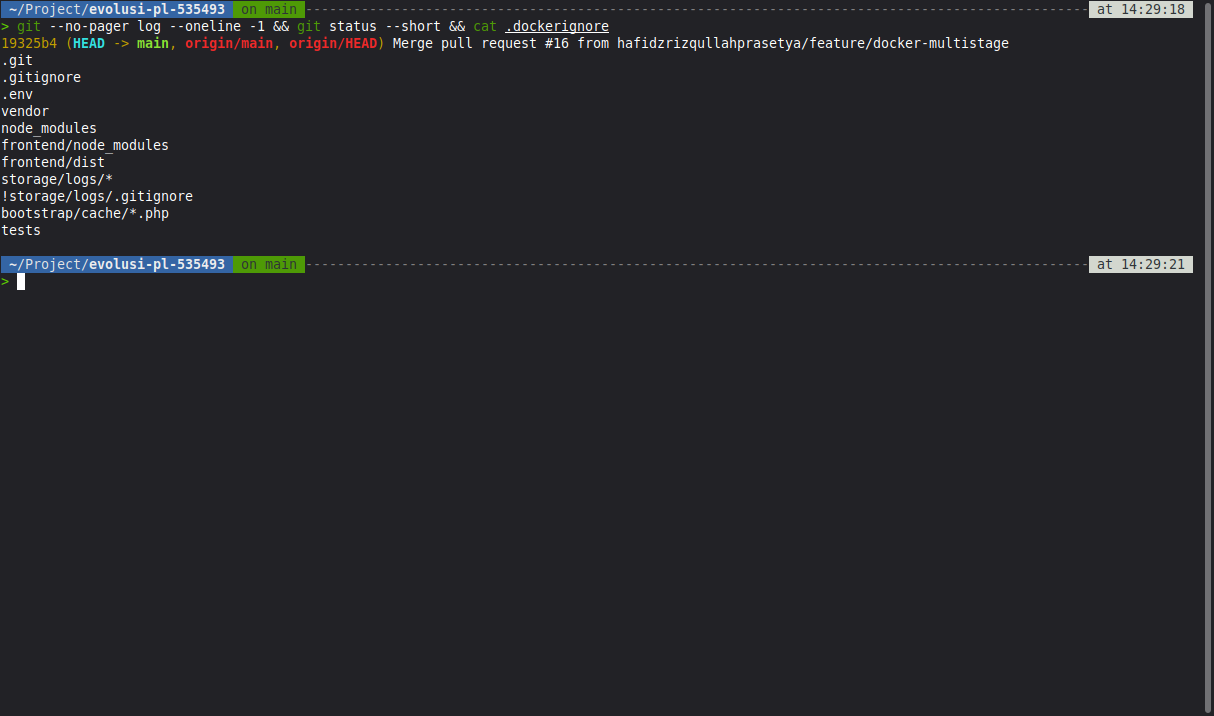
\includegraphics[width=0.98\linewidth,keepaspectratio]{images/ss-01-dockerignore.png}}
    \caption{Commit terakhir di \texttt{main} dan isi \texttt{.dockerignore} di terminal.}
    \label{fig:dockerignore}
\end{figure}

\section{Urutan Instruksi agar Cache Bekerja (Soal 3)}
Pada tahap \texttt{builder}, urutannya sebagai berikut:
\begin{enumerate}
    \item \texttt{COPY composer.json composer.lock ./} hanya menyalin dua berkas daftar dependensi;
    \item \texttt{RUN composer install --no-dev ...} memasang dependensi berdasarkan dua berkas itu;
    \item \texttt{COPY . .} baru menyalin seluruh kode aplikasi;
    \item \texttt{RUN composer dump-autoload --optimize --no-dev} membuat ulang autoloader setelah kode ada.
\end{enumerate}
Dengan urutan ini, layer \texttt{composer install} hanya dibangun ulang jika \texttt{composer.json} atau \texttt{composer.lock} berubah. Mengubah controller, route, atau view hanya membatalkan cache mulai dari \texttt{COPY . .}. Kalau \texttt{COPY . .} ditaruh sebelum \texttt{composer install}, setiap perubahan satu huruf di kode akan memaksa Composer memasang ulang semua paket. Opsi \texttt{--no-scripts} dipakai karena pada titik itu kode aplikasi, termasuk berkas \texttt{artisan}, belum ada di image.

\section{Bukti Cache Build (Soal 4)}
Build dijalankan tiga kali dengan perintah \texttt{time} supaya total waktunya tercetak di terminal. Image dari Dockerfile ini pernah dibangun saat Tugas 5 dan masih tersimpan di laptop, jadi layer lamanya bisa saja langsung terpakai. Supaya build pertama benar-benar dimulai dari nol, build pertama memakai \texttt{--no-cache}. Build kedua dan ketiga memakai perintah biasa.

\subsection{Build Pertama}
\begin{lstlisting}[style=bashstyle,caption={Build pertama tanpa cache.}]
time docker build --no-cache -t evolusi-pl-535493:tugas4 .
\end{lstlisting}

Build pertama selesai dalam 54,128 detik (Gambar \ref{fig:build1}). Langkah terlama adalah \texttt{RUN cp .env.example ...} di tahap akhir (28,0 detik), pemasangan ekstensi \texttt{bcmath} (20,5 detik), dan \texttt{composer install} (10,0 detik).

\begin{figure}[H]
    \centering
    \customfbox{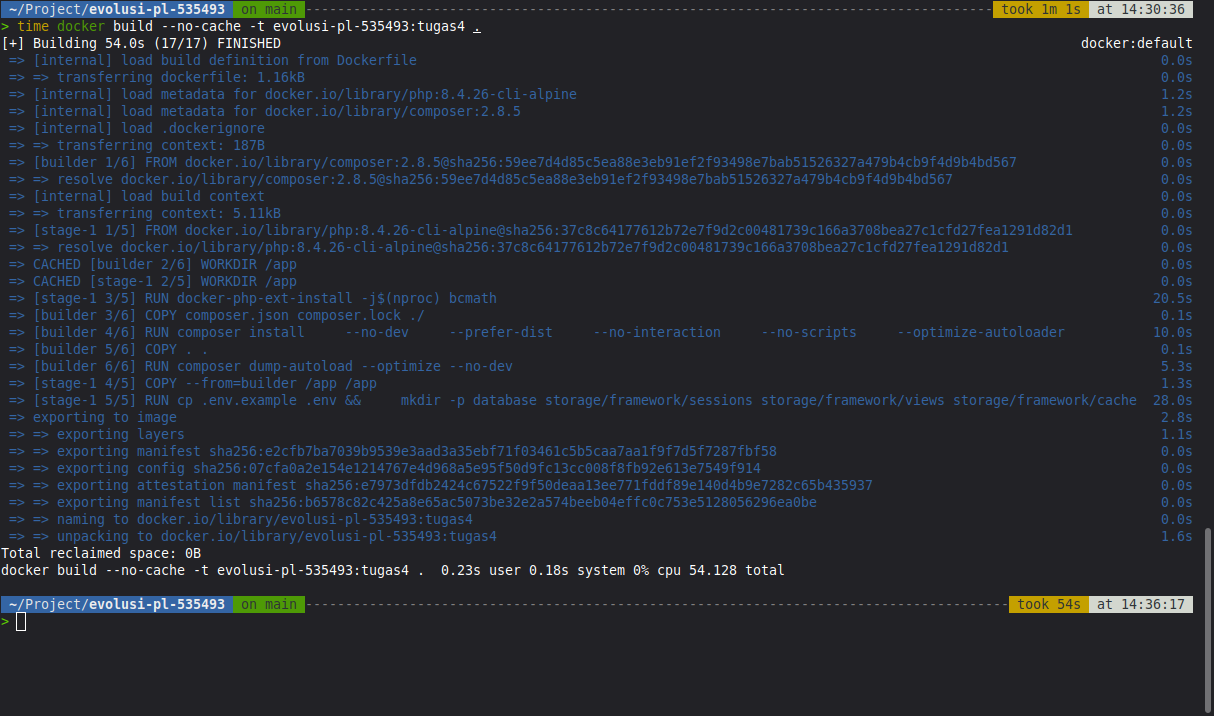
\includegraphics[width=0.98\linewidth,keepaspectratio]{images/ss-02-build-pertama.png}}
    \caption{Build pertama dengan \texttt{--no-cache}: 54,128 detik.}
    \label{fig:build1}
\end{figure}

\subsection{Build Kedua Tanpa Perubahan}
Perintah yang sama dijalankan lagi tanpa \texttt{--no-cache} dan tanpa mengubah berkas apa pun. Semua langkah bertanda \texttt{CACHED}, dan build selesai dalam 1,584 detik (Gambar \ref{fig:build2}). Waktu yang tersisa hampir seluruhnya dipakai untuk membaca metadata image dasar.

\begin{figure}[H]
    \centering
    \customfbox{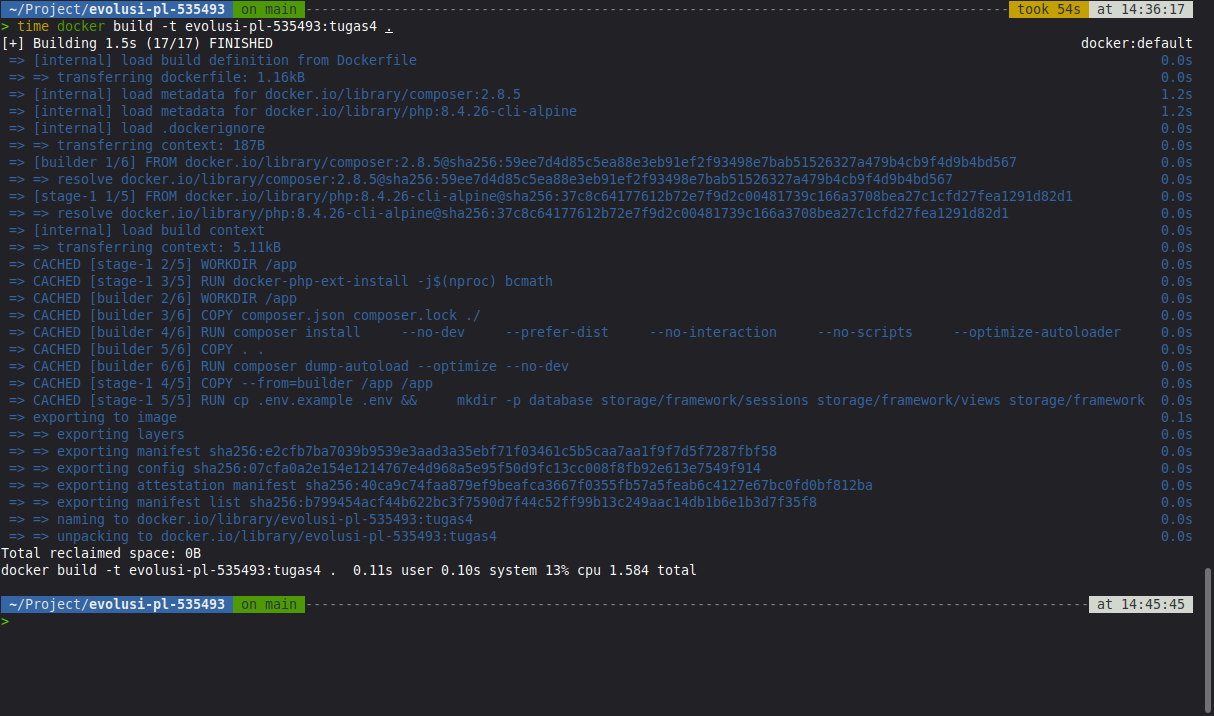
\includegraphics[width=0.98\linewidth,keepaspectratio]{images/ss-03-build-kedua.png}}
    \caption{Build kedua tanpa perubahan: semua langkah \texttt{CACHED}, 1,584 detik.}
    \label{fig:build2}
\end{figure}

\subsection{Build Ketiga Setelah Satu Huruf Diubah}
Satu huruf di \texttt{routes/web.php} diubah, yaitu teks \texttt{"IP semester"} menjadi \texttt{"IP Semester"}. Perubahan itu terlihat di \texttt{git diff} pada Gambar \ref{fig:build3}, lalu build dijalankan lagi. Build ketiga selesai dalam 26,797 detik. Layer \texttt{COPY composer.json composer.lock}, \texttt{composer install}, dan \texttt{bcmath} tetap \texttt{CACHED}. Yang dijalankan ulang hanya langkah mulai dari \texttt{COPY . .}, karena isi kode berubah. Setelah screenshot diambil, perubahan satu huruf itu dikembalikan dengan \texttt{git checkout routes/web.php}, jadi tidak ada yang di-commit.

\begin{figure}[H]
    \centering
    \customfbox{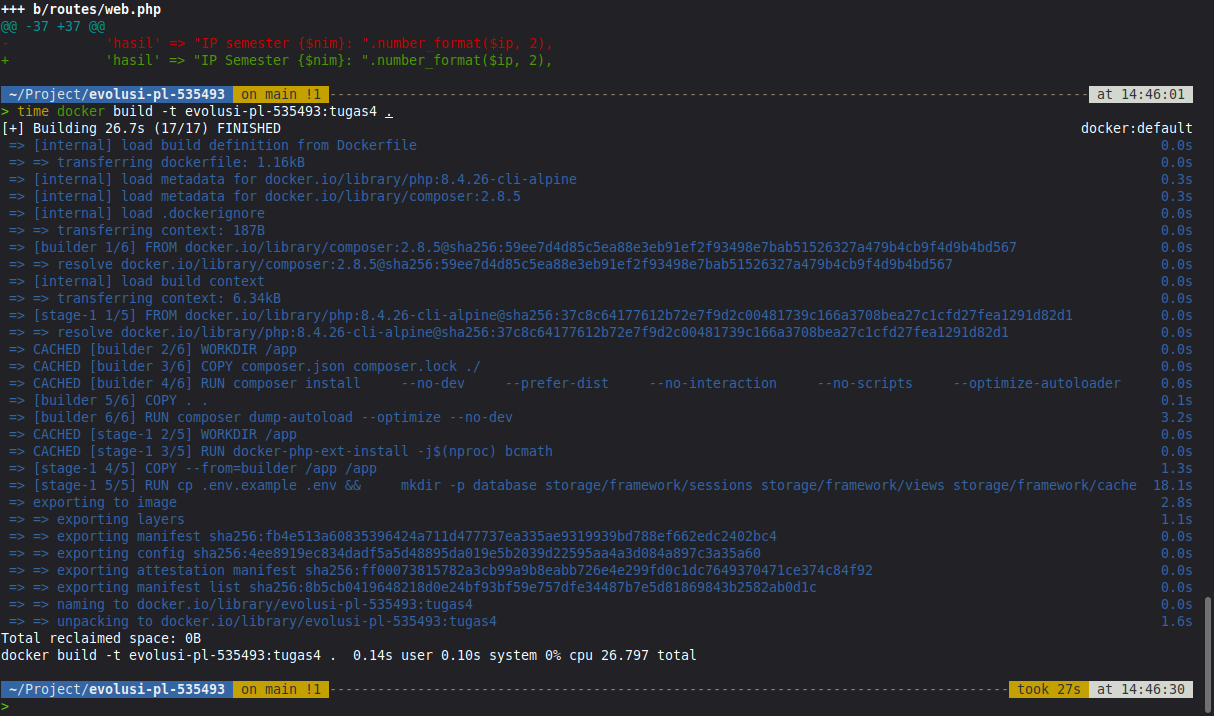
\includegraphics[width=0.98\linewidth,keepaspectratio]{images/ss-04-build-ketiga.png}}
    \caption{Perubahan satu huruf di \texttt{routes/web.php} dan build ketiga: 26,797 detik.}
    \label{fig:build3}
\end{figure}

\subsection{Perbandingan Ketiga Build}\label{sub:banding}
Tabel \ref{tab:build} merangkum waktu tiap langkah yang dibaca dari output build di Gambar \ref{fig:build1} sampai \ref{fig:build3}.

\begin{table}[!htbp]
    \centering
    \caption{Waktu langkah build (detik).}
    \label{tab:build}
    \small
    \begin{tabular}{>{\raggedright\arraybackslash}p{6.4cm}rrr}
        \toprule
        Langkah & Build 1 & Build 2 & Build 3 \\
        \midrule
        \texttt{RUN docker-php-ext-install bcmath} & 20,5 & \texttt{CACHED} & \texttt{CACHED} \\
        \texttt{COPY composer.json composer.lock} & 0,1 & \texttt{CACHED} & \texttt{CACHED} \\
        \texttt{RUN composer install} & 10,0 & \texttt{CACHED} & \texttt{CACHED} \\
        \texttt{COPY . .} & 0,1 & \texttt{CACHED} & 0,1 \\
        \texttt{RUN composer dump-autoload} & 5,3 & \texttt{CACHED} & 3,2 \\
        \texttt{COPY --from=builder /app /app} & 1,3 & \texttt{CACHED} & 1,3 \\
        \texttt{RUN cp .env.example .env \&\& ...} & 28,0 & \texttt{CACHED} & 18,1 \\
        \midrule
        Total (\texttt{time}) & 54,128 & 1,584 & 26,797 \\
        \bottomrule
    \end{tabular}
\end{table}

Build ketiga sekitar dua kali lebih cepat daripada build pertama. Penghematannya datang dari \texttt{bcmath} dan \texttt{composer install} yang tidak dijalankan ulang, sekitar 30 detik. Sisa waktunya hampir seluruhnya dipakai oleh langkah terakhir. Langkah itu harus dijalankan ulang karena layer sebelumnya (\texttt{COPY --from=builder}) ikut berubah, dan di dalamnya ada \texttt{chown -R www-data:www-data /app} yang mengubah pemilik setiap berkas, termasuk seluruh isi \texttt{vendor}. Jika ingin build ketiga lebih cepat lagi, kepemilikan bisa langsung diatur saat menyalin dengan \texttt{COPY --chown=www-data:www-data --from=builder /app /app} \cite{dockerfile-ref}. Perubahan itu belum saya terapkan di tugas ini.

\section{Container Berjalan di Browser (Soal 5)}
Container dijalankan dari image hasil build ketiga. Port 8000 di laptop sudah dipakai aplikasi lain, jadi port 8000 milik container dipetakan ke port 8081 di host:
\begin{lstlisting}[style=bashstyle,caption={Menjalankan container.}]
docker run -d --name evolusi-pl-tugas4 -p 8081:8000 evolusi-pl-535493:tugas4
\end{lstlisting}

Gambar \ref{fig:browser} memperlihatkan browser yang membuka \texttt{http://localhost:8081/api/tugas} di sebelah kiri dan output \texttt{docker ps} di sebelah kanan. Container \texttt{evolusi-pl-tugas4} berstatus \texttt{Up 54 seconds (healthy)}, artinya \texttt{HEALTHCHECK} sudah berhasil memanggil \texttt{/api/tugas}. Pemetaan port \texttt{0.0.0.0:8081->8000/tcp} juga terlihat.

\begin{figure}[H]
    \centering
    \customfbox{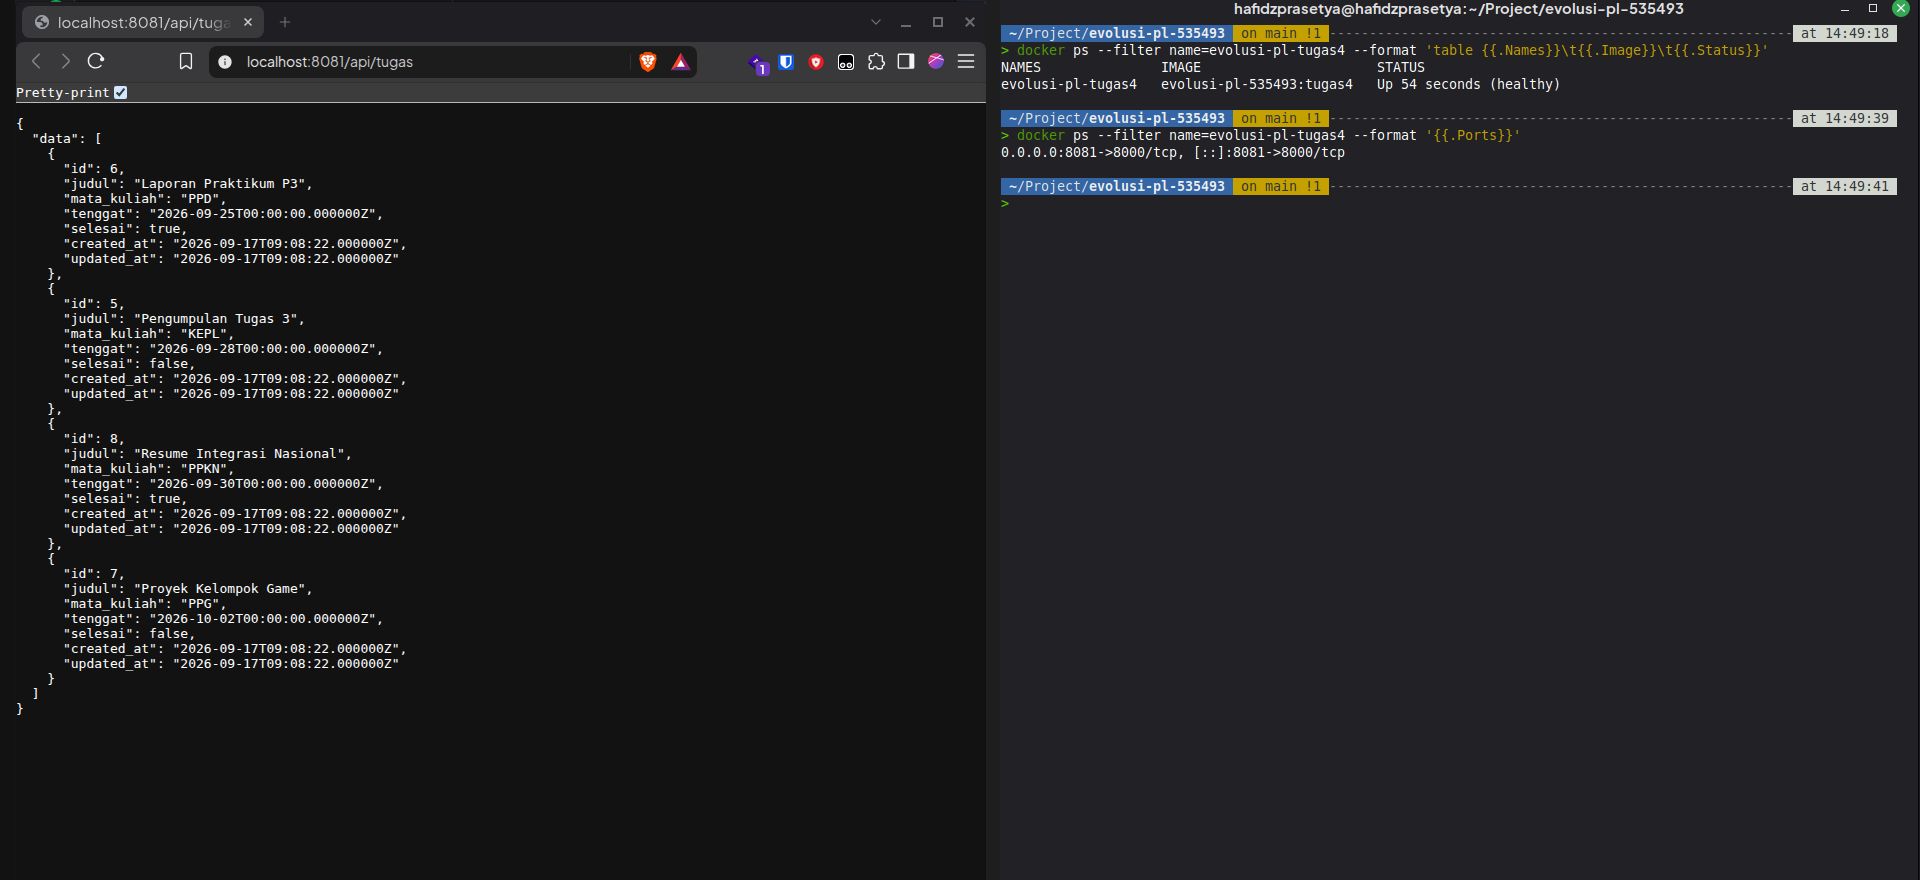
\includegraphics[width=0.98\linewidth,keepaspectratio]{images/ss-05-browser-docker-ps.png}}
    \caption{Browser membuka \texttt{/api/tugas} dari container, dan \texttt{docker ps} menunjukkan status \textit{healthy} serta port 8081.}
    \label{fig:browser}
\end{figure}

\section{Uji API dengan Postman (Soal 6)}
Di Postman, permintaan \texttt{GET http://localhost:8081/api/tugas} dikirim. Endpoint ini sama dengan yang dipakai frontend Vue pada tugas sebelumnya. Hasilnya ada di Gambar \ref{fig:postman}: status \texttt{200 OK}, waktu respons 14 ms, ukuran 1,02 KB, dan isi JSON berupa objek \texttt{data} yang berisi daftar tugas lengkap dengan \texttt{id}, \texttt{judul}, \texttt{mata\_kuliah}, \texttt{tenggat}, dan \texttt{selesai}.

\begin{figure}[H]
    \centering
    \customfbox{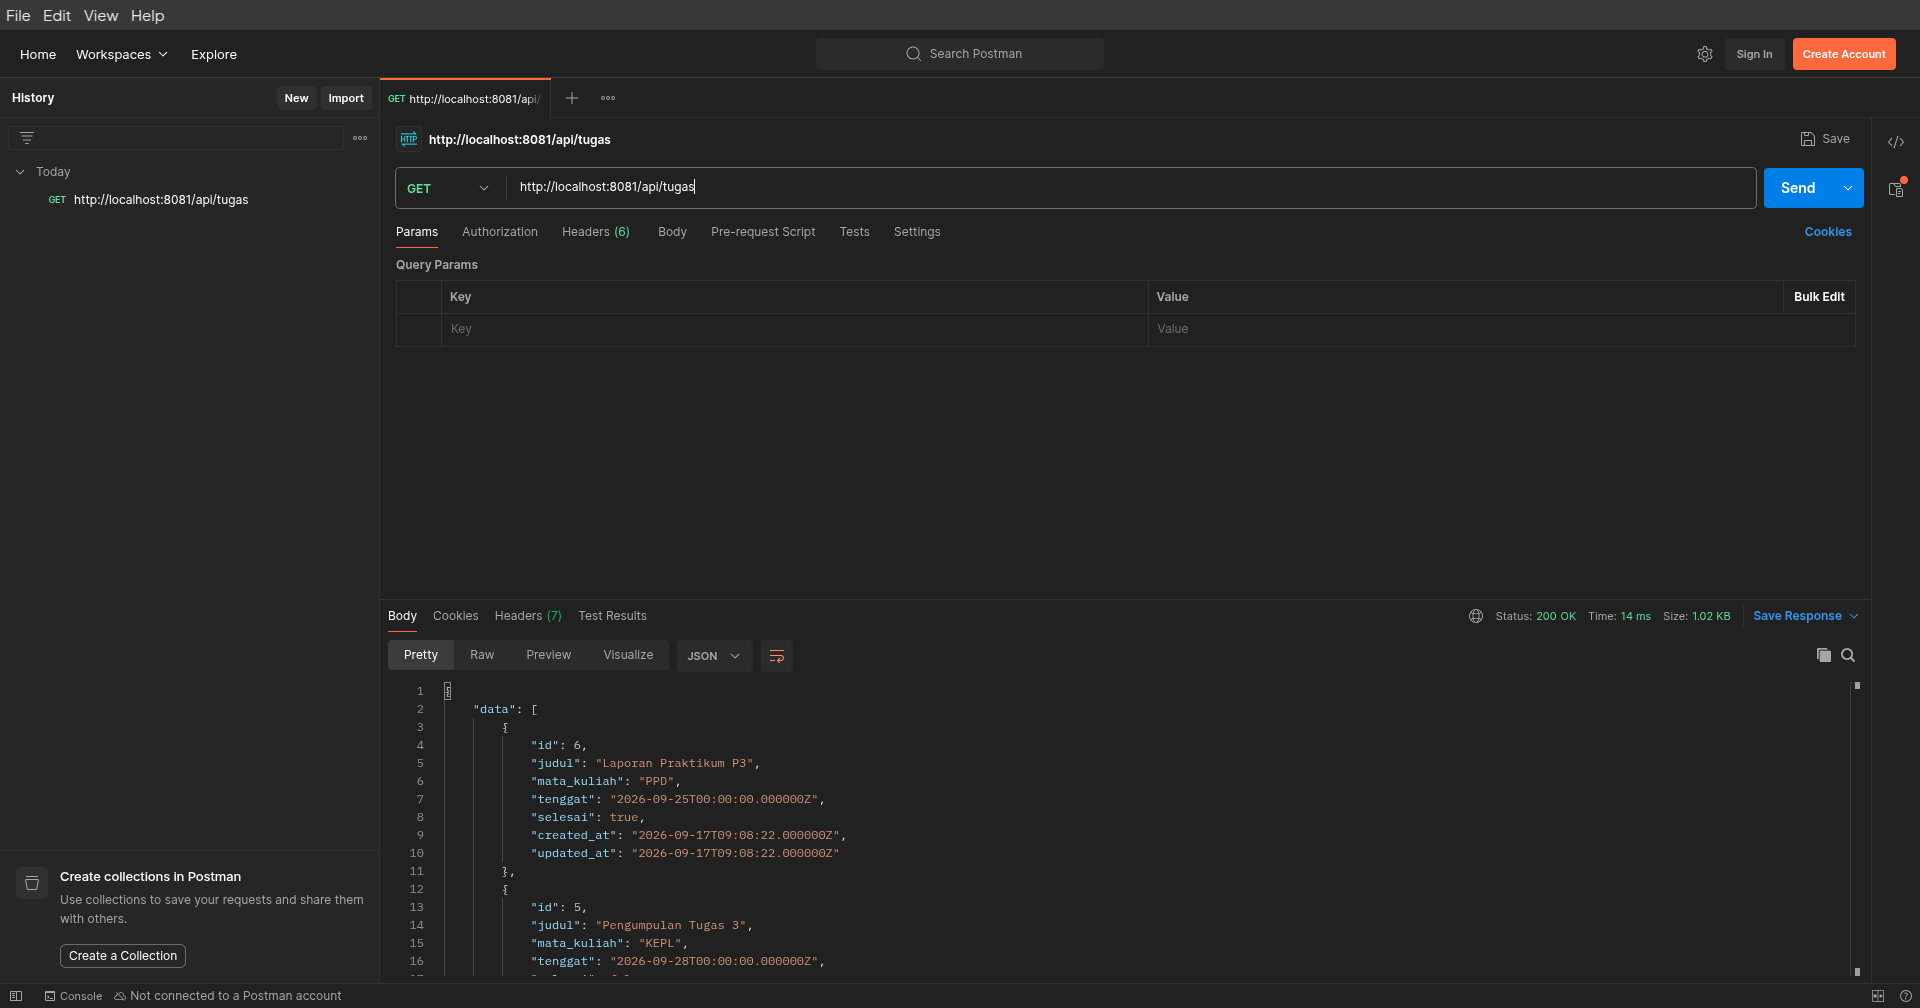
\includegraphics[width=0.98\linewidth,keepaspectratio]{images/ss-06-postman.png}}
    \caption{Postman memanggil \texttt{GET http://localhost:8081/api/tugas} dengan status 200 OK dan balasan JSON.}
    \label{fig:postman}
\end{figure}

Empat data tugas di balasan itu berasal dari berkas \texttt{database/database.sqlite} di laptop. Berkas itu diabaikan Git lewat \texttt{database/.gitignore}, tetapi tidak tercantum di \texttt{.dockerignore}, sehingga ikut tersalin oleh \texttt{COPY . .}. Hal ini juga terlihat dari pesan \texttt{Nothing to migrate} pada Gambar \ref{fig:build3}, karena tabelnya sudah ada di berkas tersebut. Untuk image produksi, pola \texttt{database/*.sqlite} sebaiknya ditambahkan ke \texttt{.dockerignore} agar data lokal tidak terbawa ke image.

\clearpage

\chapter{Kendala dan Solusi}
\begin{enumerate}
    \item Port 8000 di laptop sudah dipakai aplikasi lain, sehingga container dipetakan ke port 8081 (\texttt{-p 8081:8000}).
    \item Postman belum terpasang di laptop. Postman dipasang lewat Flatpak dari Flathub, lalu dipakai dalam mode \textit{Lightweight API Client} yang tidak memerlukan akun.
    \item Build ketiga hanya sekitar dua kali lebih cepat daripada build pertama, karena langkah \texttt{chown -R} di tahap akhir tetap dijalankan ulang setiap kali kode berubah. Penyebab dan usulan perbaikannya dibahas di Subbab \ref{sub:banding}.
\end{enumerate}

\clearpage

\chapter{Kesimpulan}
\begin{enumerate}
    \item \texttt{Dockerfile} multi-stage dan \texttt{.dockerignore} sudah ter-commit di repositori \texttt{evolusi-pl-535493}. \texttt{.dockerignore} mengecualikan \texttt{.git}, \texttt{.env}, \texttt{vendor}, dan \texttt{node\_modules}, sehingga context build hanya sekitar 5 kB.
    \item \texttt{composer.json} dan \texttt{composer.lock} disalin dan dipasang sebelum \texttt{COPY . .}, sehingga perubahan kode tidak memicu pemasangan ulang dependensi.
    \item Build pertama tanpa cache memakan 54,128 detik, build ulang tanpa perubahan 1,584 detik, dan build setelah satu huruf diubah 26,797 detik. Pada build ketiga, \texttt{composer install} dan \texttt{bcmath} tetap \texttt{CACHED}.
    \item Container berjalan dengan status \textit{healthy} di port 8081 dan bisa dibuka dari browser.
    \item Endpoint \texttt{GET /api/tugas} membalas \texttt{200 OK} dengan JSON saat dipanggil dari Postman di luar container.
\end{enumerate}

\clearpage

\begin{thebibliography}{99}
\addcontentsline{toc}{chapter}{Daftar Pustaka}

\bibitem{dockerfile-ref}
Docker Inc., ``Dockerfile reference,'' Docker Docs, 2026. [Daring]. Tersedia: \url{https://docs.docker.com/reference/dockerfile/}. [Diakses: 18-Nov-2026].

\bibitem{docker-cache}
Docker Inc., ``Docker build cache,'' Docker Docs, 2026. [Daring]. Tersedia: \url{https://docs.docker.com/build/cache/}. [Diakses: 18-Nov-2026].

\bibitem{docker-context}
Docker Inc., ``Build context,'' Docker Docs, 2026. [Daring]. Tersedia: \url{https://docs.docker.com/build/concepts/context/}. [Diakses: 18-Nov-2026].

\bibitem{docker-ports}
Docker Inc., ``Publishing and exposing ports,'' Docker Docs, 2026. [Daring]. Tersedia: \url{https://docs.docker.com/get-started/docker-concepts/running-containers/publishing-ports/}. [Diakses: 18-Nov-2026].

\bibitem{postman-request}
Postman Inc., ``Send API requests and get response data in Postman,'' Postman Docs, 2026. [Daring]. Tersedia: \url{https://learning.postman.com/docs/sending-requests/create-requests/request-basics/}. [Diakses: 18-Nov-2026].

\end{thebibliography}

\end{document}
